\begin{figure}[H]
    \centering
    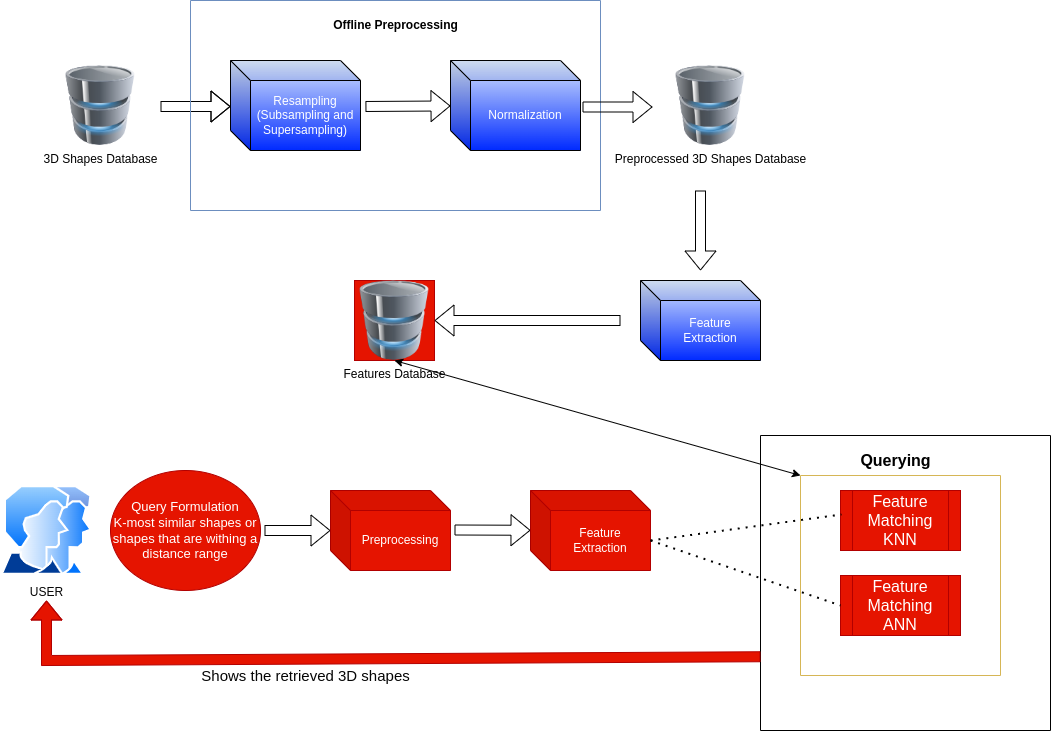
\includegraphics[width=0.9\textwidth]{assets/pipeline.png}
    \caption{Multimedia retrieval system pipeline}
    \label{fig:mr-pipeline}
\end{figure}

\begin{table}
    \caption{Global Notations}
    \centering
    \resizebox{\textwidth}{!}{
        \begin{tabular}{|c|c|c|c|}
            \hline
            Name & Notation & Description & Formula \\ [0.5ex]
            \hline\hline

            \newtag{3D Point}{3d_point_not} & $p$ & A tuple representing coordinates in 3D & $p = (x,y,z)$ \\
            \hline
            
            \newtag{Normal}{normal_not} & $|| \cdot ||$ & The distance from the origin & $||p|| = \sqrt{p_x^2 + p_y^2 + p_z^2}$ \\
            \hline      
            
            \newtag{Triangle}{triangle_not} & $\mathcal{T}$ & A set of 3 points forming a triangle & $\mathcal{T} = \{p_1, p_2, p_3\}$ \\
            \hline

            \newtag{Tetrahedron}{tetrahedron_not} & $\mathcal{T}h$ & A set of 4 points forming a tetrahedron & $\mathcal{T}h = \{p_1, p_2, p_3, p_4\}$ \\
           \hline
           \newtag{Tetrahedron with}{tetrahedron_origin_not} & \multirow{2}{*}{$\mathcal{T}h_O$} & A set of 3 points forming a tetrahedron  & \multirow{2}{*}{$\mathcal{T}h_O = \{p_1, p_2, p_3, O\}$} \\
              a vertex in origin & & where the 4th point is the origin $O = (0,0,0)$ & \\
          \hline
            
           \newtag{Triangle center}{triangle_center_not} & $\mathbf{C}_{\mathcal{T}}$ & The center of the triangle & $\mathbf{C}_{\mathcal{T}} = (\frac{p_{1_x} + p_{2_x} + p_{3_x}}{3}, \frac{p_{1_y} + p_{2_y} + p_{3_y}}{3}, \frac{p_{1_z} + p_{2_z} + p_{3_z}}{3} )$ \\
           \hline      
            
           Unsigned tetrahedron & \multirow{2}{*}{\newtag{$Vol_{\mathcal{T}h}$}{tetrahedron_volume_not}} & \multirow{2}{*}{The volume of the tetrahedron $\mathcal{T}h$} & \multirow{2}{*}{$Vol_{\mathcal{T}h} = \frac{1}{6} \cdot (p_1 - p_4) \cdot ((p_2 - p_4) \times (p_3 - p_4))$} \\
           volume & & & \\
           \hline   
            
           Triangle area & \newtag{$A_{\mathcal{T}}$}{triangle_area_not} & The area of the triangle $\mathcal{T}$ & $A_{\mathcal{T}} = \frac{1}{2} \cdot ||(p_2 - p_1) \times (p_3 - p_1)|| $ \\
           \hline   
            
           Vertices & \newtag{$V$}{vertices_not} & A set of 3D points & $V = \{v_1, ..., v_N\}$ \\
           \hline      
             
           Faces & \newtag{$F$}{faces_not} & A set of triples of indexes & $F = \{(i,j,k), ..., (l,m,n)\}$ \\
           \hline      
            
           \multirow{2}{*}{Shape} &\multirow{2}{*}{\newtag{$\mathcal{S}$}{shape_not}} & A set of vertices and a set of & \multirow{2}{*}{$\mathcal{S} = (V_\mathcal{S}, F_\mathcal{S})$} \\
           & & faces containing vertices indexes & \\
           \hline      
            
            Barycenter & \newtag{$b_{\mathcal{S}}$}{barycenter_not} & The geometric center of shape $\mathcal{S}$ & $b_{\mathcal{S}} = \frac{1}{N} \sum_{i=1}^N \mathbf{C}_{\mathcal{T}_i} \cdot A_{\mathcal{T}_i}$  \\
           \hline      

           \multirow{2}{*}{\newtag{All the matrices}{matrices_class_not}} & \multirow{4}{*}{$\mathbb{M}_{n,m}(\cdot)$} & e.g. $\mathbb{M}_{2,3}(\mathbb{R})$ represents & \multirow{4}{*}{$\mathbb{M}_{n,m}(\cdot) = 
            \begin{pmatrix}
                a_{1,1} & \cdots & a_{1,m} \\
                \vdots & \ddots & \vdots \\
                a_{n,1} & \cdots & a_{n,m} \\
            \end{pmatrix}
           $} \\
           & & all the matrices & \\
           \multirow{2}{*}{of size $n \times m$} & & with 2 rows and 3 columns & \\
           & & containing only real numbers & \\
           \hline
            
           \newtag{Identity Matrix}{identity_matrix_not} & $\mathbb{I}_N$ & The $N\times N$ identity matrix & 
            
           $\mathbb{I}_N = 
             \begin{pmatrix}
                  1 & 0 &\cdots & 0 \\
                  0 & 1 &\cdots & 0 \\
                 \vdots &\vdots& \ddots & \vdots \\
                 0 & 0 & \cdots & 1
             \end{pmatrix}$ \\
           \hline      
            
           \newtag{Matrix transposition}{matrix_transposition_not} & $(\cdot)^T$ & Transposing a matrix & Let $A=(a_{i,j})$ then $A^T=(a_{j,i})$\\
           \hline

           \newtag{Covariance}{cov_x_y_not} & \multirow{3}{*}{$cov(x,y)$} & An indicator of the spread of the vertices & $cov(x,y) = \frac{1}{N-1} \sum_{i=1}^N (x_i - \bar{x}) \cdot (y_i - \bar{y})$, \\
           of $x$ coordinate & & along $x$ coordinate axis & where $\bar{x} = \frac{1}{N} \sum_{i=1}^N x_i$\\
           w.r.t. $y$ coordinate & & w.r.t. the spread along the $y$ axis & $\bar{y} = \frac{1}{N} \sum_{i=1}^N y_i$ \\
           \hline      
            
           \newtag{Covariance matrix}{cov_shape_not} & \multirow{3}{*}{$Cov(V_{\mathcal{S}})$} & The matrix describing the spread & \multirow{3}{*}{ $Cov(V_{\mathcal{S}}) = \begin{pmatrix}
                    cov(x,x) & cov(x,y) & cov(x,z)\\
                    cov(y,x) & cov(y,y) & cov(y,z)\\
                    cov(z,x) & cov(z,y) & cov(z,z)\\ 
              \end{pmatrix}$}
              \\
            of shape $\mathcal{S}$ & & of vertices w.r.t. coordinate axes & \\
            & & & \\
           \hline      
            
           \newtag{Eigenvalue}{eigval_shape_not} & \multirow{2}{*}{$\lambda$} & The variability of the data in the direction & \multirow{2}{*}{$det(Cov(V_{\mathcal{S}}) - \lambda \cdot \mathbb{I}_N) = 0$} \\
           of shape $\mathcal{S}$ & & corresponding to the eigenvectors & \\
           \hline      
            
           \newtag{Eigenvector}{eigvec_shape_not} & \multirow{2}{*}{$v_{\lambda}$} & The direction vectors in which & \multirow{2}{*}{$Cov(V_{\mathcal{S}}) \cdot \overrightarrow{v_{\lambda}} = \lambda \cdot \overrightarrow{v_{\lambda}}$} \\
           of shape $\mathcal{S}$ & & the data is spread the most & \\
           \hline      
            
           Flipping axis & \multirow{3}{*}{\newtag{$f_i$}{flip_axis_not}} & The weighted difference & \multirow{2}{*}{$f_i = \sum\limits_{j=1}^M  sign({C}_{\mathcal{T}_j}^i) \cdot ({C}_{\mathcal{T}_j}^i)^2$} \\
           component & & of the amount of vertices & \\
            of shape $\mathcal{S}$ & & on the positive and negative side of axis $i$ & where $|F_{\mathcal{S}}| = M$ \\ 
           \hline      
            
           Re-scaling & \multirow{2}{*}{\newtag{$\sigma_{unit}(\mathcal{S})$}{rescale_not}} & The unit cube re-scaling factor & $\sigma_{unit}(\mathcal{S}) = \frac{1}{m}$\\
           unit cube factor & & of a shape $\mathcal{S}$ & $m = max(|x_{max} - x_{min}|, |y_{max} - y_{min}|, |z_{max} - z_{min}|)$ \\ 
           \hline
           
           \multirow{2}{*}{\newtag{LP norm}{lp_norm}} & \multirow{2}{*}{$L_p(\cdot, \cdot)$} & \multirow{2}{*}{A distance function between two vectors} & $L_p(\overrightarrow{x},\overrightarrow{y}) = \left( \sum_{i = 1}^n \left| x_i - y_i \right| ^p \right)^{\frac{1}{p}}$ \\
           & & & $L_{\infty}(\overrightarrow{x},\overrightarrow{y}) = \max_{i = 1}^n \left| x_i - y_i \right|$ \\
           
           \hline
           \newtag{Cosine distance}{cos_dist} & $d_{cos}(\cdot, \cdot)$ & A distance function between two vectors& $d_{cos}(\overrightarrow{x}, \overrightarrow{y}) = 1 - \frac{\overrightarrow{x} \cdot \overrightarrow{y}}{||\overrightarrow{x}||\cdot ||\overrightarrow{y}||}$ \\
           
            \hline
            \multirow{2}{*}{\newtag{Mahalanobis Distance}{mahalanobius_dist}} & \multirow{2}{*}{$d_{mahalanobis}(\cdot, \cdot)$} & \multirow{2}{*}{A distance function between two vectors}  & $d_{mahalanobis}(\overrightarrow{x}, \overrightarrow{y}) = \sqrt{(\overrightarrow{x} - \overrightarrow{y})^T Cov^{-1}(X) (\overrightarrow{x} - \overrightarrow{y})}$\\
            & & & where $X$ is the set of all points in the space \\
            \hline
           
            \multirow{4}{*}{\newtag{Earth's Mover's Distance}{emd_dist}} & \multirow{4}{*}{$emd(\cdot,\cdot)$} & \multirow{2}{*}{A distance function} & $emd(A,B) = \min\limits_{F} \frac{\sum_{i=1}^{n} \sum_{j=1}^{m} f_{i, j} d_{i, j}}{\sum_{i=1}^{n} \sum_{j=1}^{m} f_{i,j}}$ \\
            & & & where $F=\{f_{i,j}\}$, with $f_{i,j}$ \\
            & & \multirow{2}{*}{between two histograms} & the flow between bin $i$ of $A$ and bin $j$ of $B$ \\
            & & & and $d_{i,j}$ the distance between the bins (see \cite{rubner_emd_2000})\\
            \hline
            
            \multirow{4}{*}{\newtag{Kullback-Leibler Divergence}{KL_dist}} & \multirow{4}{*}{$d_{KL}(\cdot, \cdot)$} & \multirow{2}{*}{A distance function between} & $d_{KL}(A, B) = \sum_{i=1}^n (a_i - b_i) \log \left( \frac{a_i}{b_i} \right)$ \\
            & & & where $A$ and $B$ are discrete random variables\\
            & & \multirow{2}{*}{two probability distributions} & where the probability of the event $i$ equals to \\
            & & & $a_i$ and $b_i$ respectively (see \cite{kullback1951information})\\
            \hline
            
        \end{tabular}
    }
    \label{tab:notations}
\end{table}
Table \ref{tab:notations} describes all notations used throughout the report. We use the notation $\overrightarrow{p_1} \times \overrightarrow{p_2}$ for the cross product between two vectors; $\alpha \cdot \overrightarrow{p_1}$ for scalar multiplication; $\overrightarrow{p_1} \cdot \overrightarrow{p_2}$ for dot product; and $A \cdot B$ for matrix multiplication. Table \ref{tab:code_tools} presents all the dependent libraries of our system.

\begin{table}
    \caption{Code Tools}
    \centering
    \resizebox{\textwidth}{!}{
        \begin{tabular}{|c|c|c|c|}
            \hline
            Name & Description & Citation/Website \\
            [0.5ex]
            \hline\hline
                \newtag{Python 3}{python_t} &
                Base programming language for the project &
                \cite{10.5555/1593511} \\
            \hline
                \newtag{PyMeshLab}{pymeshlab_t} & 
                Python interface to \ref{meshlab_t} &
                \cite{pymeshlab} \\
            \hline
                \newtag{MeshLab}{meshlab_t} &
                System for processing and editing 3D shapes &
                \cite{MeshLab} \\
            \hline
                \newtag{PyVista}{pyvista_t} &
                Visualisation of 3D Models &
                \cite{sullivan2019pyvista} \\
            \hline
                \multirow{2}{*}{\newtag{Numba}{numba_t}} &
                Speed up (some) \ref{python_t} \& \ref{np_t} functions &
                \multirow{2}{*}{\cite{lam2015numba}} \\
                & by translating them into machine code & \\
            \hline
                \newtag{NumPy}{np_t} &
                Extensive mathematical functions for \ref{python_t}, computed quickly &
                \cite{harris2020array} \\
            \hline
                \newtag{SciPy}{scipy-t} & 
                Fundamental algorithms for scientific computing &
                \cite{2020SciPy-NMeth} \\
            \hline
                \newtag{Matplotlib}{plt_t} &
                Plotting data for visualisation purposes; plots used in the report &
                \cite{Hunter:2007} \\
            \hline
                \newtag{SciencePlots}{sciplots_t} & 
                Scientific plot styles for \ref{plt_t} &
                \href{https://pypi.org/project/SciencePlots/}{pypi.org} \\
            \hline
                \newtag{PySimpleGUI}{PySimpleGUI_t} &
                Used to make the GUI for the end system &
                \href{https://www.pysimplegui.org/}{pysimplegui.org} \\
            \hline
                \newtag{Annoy}{Annoy_t} & Used to compute an index of the feature database & \href{https://pypi.org/project/annoy/1.0.3/}{pypi.org}
                \\
            \hline
        \end{tabular}
    }
    \label{tab:code_tools}
\end{table}
